\documentclass[portrait,plainboxedsections]{sciposter}

% Override font size limits
\usepackage{anyfontsize}
% Select Computer Concrete as default font
\usepackage{concrete}
% Select Computer Concrete as math font
\usepackage{concmath}
\usepackage[T1]{fontenc}
% Set default font family as serif (sciposter sets sans serif by default)
\renewcommand{\familydefault}{\rmdefault}
% ApJ style citations
\usepackage{natbib}
\usepackage{amsmath}
\usepackage{amssymb}
% For toprule
\usepackage{booktabs}
\usepackage{graphicx}
% Computer Concrete makes AAS macros show up in wrong font size; workaround
\usepackage{microtype}
%\usepackage{aas_macros}
\newcommand{\prd}{Phys. Rev. D}
% Color mixing
\usepackage{xcolor}
% \textlangle and \textrangle
\usepackage{textcomp}

\newcommand{\earlywarning}{early-warning}
\newcommand{\GW}{{\sc gw}}
\newcommand{\EM}{{\sc em}}
\newcommand{\GRB}{{\sc grb}}
\newcommand{\CBC}{{\sc cbc}}
\newcommand{\LIGO}{{\sc ligo}}
\newcommand{\LCGT}{{\sc lcgt}}
\newcommand{\GEO}{{\sc geo600}}
\newcommand{\ISCO}{{\sc isco}}
\newcommand{\SNR}{{\sc snr}}
\newcommand{\realtime}{real-time}
\newcommand{\Msun}{\ensuremath{M_{\odot}}}
\newcommand{\order}[1]{\ensuremath{\mathcal{O}[#1]}}
\newcommand{\tmpsamps}{\ensuremath{N}}
\newcommand{\numtmps}{\ensuremath{M}}
\newcommand{\numslices}{\ensuremath{S}}
% macros for number of svd basis functions
\newcommand{\SVD}{{\sc svd}}
\newcommand{\svdtmps}[1]{\ensuremath{L^#1}}
\newcommand{\numsvdtmps}{\svdtmps{s}}
% macros for sample points in slices
\newcommand{\slicesamps}[1]{\ensuremath{N^#1}}
\newcommand{\slicessamps}{\slicesamps{s}}
\newcommand{\fftblock}{\ensuremath{D}}
\newcommand{\resampsamps}{\ensuremath{N^\shortdownarrow,\, N^\shortuparrow}}
\newcommand{\fir}{{\sc fir}}
\newcommand{\fft}{{\sc fft}}
\newcommand{\fmax}{\ensuremath{f^0}}
\newcommand{\flops}{flop/s}
\newcommand{\gstlal}{{\tt gstlal}}
\newcommand{\gstreamer}{{\tt GStreamer}}
\newcommand{\numcpus}{{600}}
\newcommand{\lloid}{{\sc lloid}}
\newcommand{\TD}{{\sc td}}
\newcommand{\FD}{{\sc fd}}

% Macros for collapsing sizes of things
% From TUGboat, Volume 22 (2001), No. 4
% http://www.tug.org/TUGboat/tb22-4/tb72perlS.pdf
\def\clap#1{\hbox to 0pt{\hss#1\hss}}
\def\mathllap{\mathpalette\mathllapinternal}
\def\mathrlap{\mathpalette\mathrlapinternal}
\def\mathclap{\mathpalette\mathclapinternal}
\def\mathllapinternal#1#2{\llap{$\mathsurround=0pt#1{#2}$}} 
\def\mathrlapinternal#1#2{\rlap{$\mathsurround=0pt#1{#2}$}} 
\def\mathclapinternal#1#2{\clap{$\mathsurround=0pt#1{#2}$}}

% Colors for signal flow diagram and equation
\def\diagramcolorfir{red}
\def\diagramcolorreconstruct{blue}
\def\diagramcoloraccum{red!50!yellow}

% Redefine style for \section*
\renewcommand{\sPlainBoxSection}[1]{
  \vspace{\secskip}
    \setlength{\secboxwidth}{\columnwidth}
    \addtolength{\secboxwidth}{-1cm}
    \setlength{\fboxrule}{2pt}
    \setlength{\fboxsep}{0pt}
        \vspace{1.1ex}
          \hspace{1.1ex}{\sectionsize{#1}} \\
  \rule[10pt]{\textwidth}{2pt}
  \par\vspace{1ex}
}

% Redefine style for "Figure #" or "Table #" text in captions
\renewcommand{\mastercapstartstyle}[1]{\sc{\color{ink2!50!black}#1}}

\begin{document}

% Title banner
\begin{minipage}[t]{0.25\textwidth}
\raggedleft
{\fontsize{36}{50}\selectfont
Poster presented by

Leo Singer (lsinger@caltech.edu)

\makebox[0pt][r]{N. Fotopoulos (foton@caltech.edu)}

}
\vspace{10mm}
\begin{minipage}[b]{130mm}\raggedleft
{\PARstart{}{scan me to read in ApJ $\rightarrow$}

\fontsize{24}{36}\selectfont
\input{doi}
}\end{minipage}%

\includegraphics[width=60mm]{doi.png}%
\end{minipage}%
\hspace{0.05\textwidth}%
\begin{minipage}[t]{0.6\textwidth}
{\vspace{-8mm}\fontsize{60}{80}\selectfont%
Toward early-warning detection of gravitational

waves from of compact binary coalescence

\vspace{1em}
\fontsize{30}{40}\selectfont
	Kipp Cannon,
	Romain Cariou,
	Adrian Chapman,
	Mireia Crispin-Ortuzar,
	Nickolas Fotopoulos,
	Melissa Frei,
	Chad Hanna,
	Erin Kara,
	Drew Keppel,
	Laura Liao,
	Stephen Privitera,
	Antony Searle,
	Leo Singer, and
	Alan Weinstein

}
\end{minipage}
\vspace{1cm}


\begin{minipage}[t]{0.25\textwidth}

% FIXME: Motivation seems to be a different font size than other section headers
\section*{Motivation}
\PARstart{\color{ink1!50!black}A}{\color{ink1!50!black}s a compact binary system} loses energy to gravitational waves (\GW{}s), its
orbital separation decays, leading to a runaway inspiral with the \GW{}
amplitude and frequency increasing until the system eventually merges.

{\setlength{\parindent}{1em}
If a neutron star (\textsc{ns}) is involved, it may become tidally disrupted near
merger and fuel an electromagnetic (\EM{}) counterpart~%
\citep{shibata:2007}.  Effort from both the \GW{} and astronomy communities may make it
possible to use \GW{} observations as an early warning trigger for \EM{}
followup.

In principal, the \GW\ signal is detectable even before tidal
disruption. One may have the ambition of reporting \GW\ candidates not minutes
after merger, but seconds before.  We explore one essential ingredient of this
problem, a computationally inexpensive low-latency filtering algorithm.

}%
\begin{figure}[h]
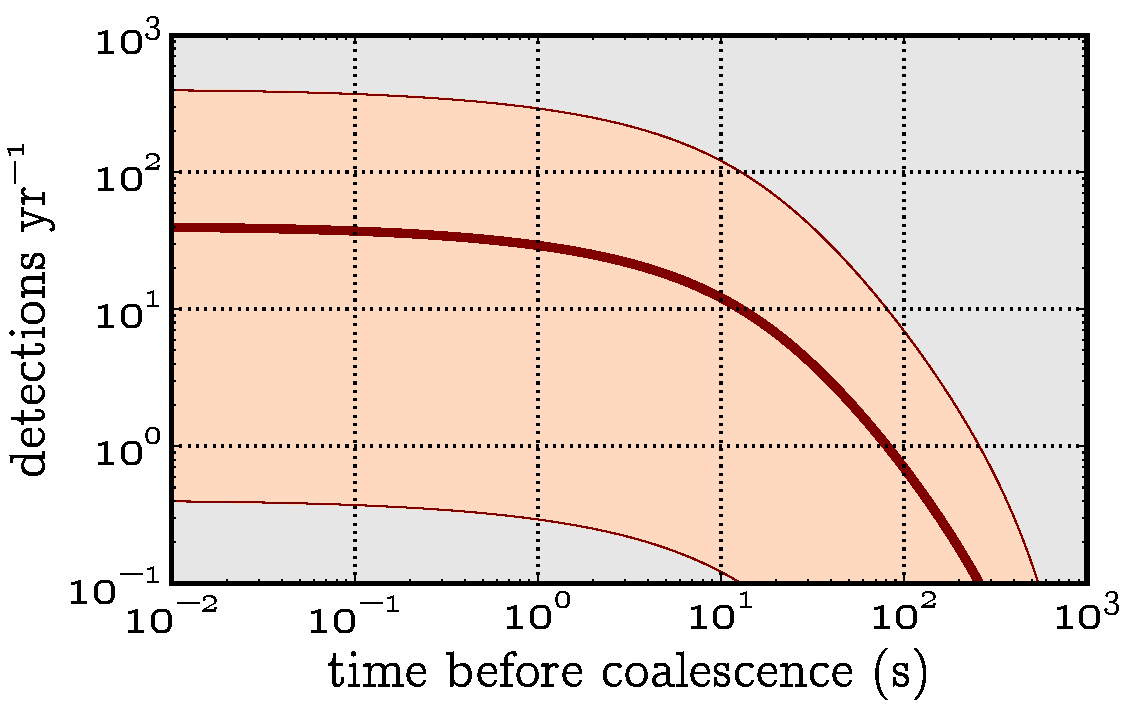
\includegraphics[width=1.05\textwidth]{figures/snr_in_time}
\caption{\label{fig:earlywarning}Expected number of {\small NS}--{\small NS}
sources detectable by Advanced {\small LIGO} a given number of seconds
before coalescence.  The heavy solid line is the most realistic yearly rate
estimate.  The shaded region represents the 5 to 95\% confidence interval
arising from uncertainty in predicted event rates~\citep{Abadie:2010p10836}.}
\end{figure}

\begin{figure}[h]
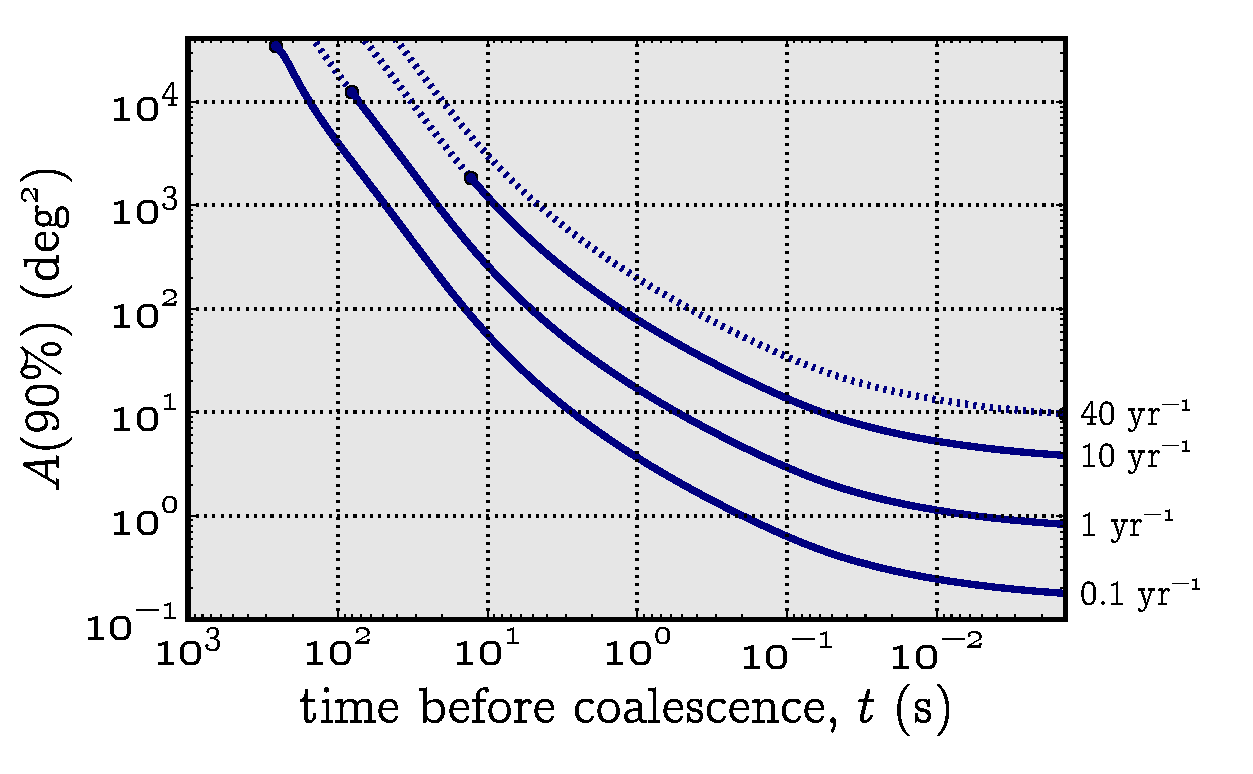
\includegraphics[width=1.15\textwidth]{figures/loc_in_time}
\caption{\label{fig:sky-localization-accuracy}Area of the 90\% confidence
region~\citep{Fairhurst2009} without a galaxy catalog prior as a function of time before coalescence for sources with anticipated
detectability rates of \oldstylenums{40}, \oldstylenums{10}, \oldstylenums{1}, and \oldstylenums{0.1}~yr$^{-1}$. The heavy dot indicates
the time at which the accumulated \SNR\ exceeds a threshold of~\oldstylenums{8}.}
\end{figure}

There were a number of sources of latency associated with the search for
\CBC{} signals in the joint \LIGO{}/Virgo data-taking run \textsc{s}\oldstylenums{6}/\textsc{vsr}\oldstylenums{3}~\citep{HugheyGWPAW2011}:

\begin{itemize}
\item Data acquisition and aggregation ($\gtrsim$100~ms)

\item Data conditioning ($\sim$1~min)

\item Trigger generation (2--5~min)

\item Alert generation (2--3~min)

\item Human validation (10--20~min)

\end{itemize}

\end{minipage}%
\hspace{0.05\textwidth}%
\begin{minipage}[t]{0.4\textwidth}

\section*{The LLOID algorithm}

\PARstart{\color{ink1!50!black}S}{\color{ink1!50!black}earches for inspiral signals} employ matched
filter banks.
Our algorithm, called \lloid{}~(Low Latency Online Inspiral Detection),
consists of a network of orthogonal filters that closely approximates the matched filters, but with greatly reduced computational cost and with nearly zero latency.
Similar to the multi-band approach of \citet{Buskulic2010}, we chop the templates into
disjoint \emph{time slices} that are processed at reduced sample rates.
Then, we reduce the number of filters using the singular value decomposition (\textsc{svd}) to factor the time-sliced templates
into orthogonal \textsc{fir} filters and a reconstruction matrix~\citep{Cannon:2010p10398}.
\begin{figure}[h!]
	\begin{center}
		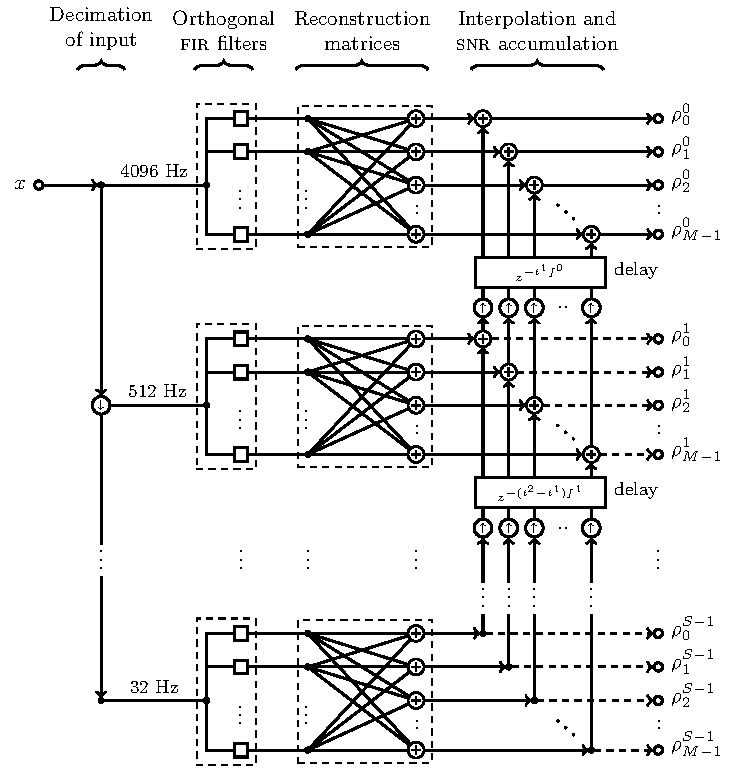
\includegraphics[width=\textwidth]{figures/lloid-diagram}
		\caption{\label{fig:pipeline} Schematic of \lloid{} algorithm.
		Circles with arrows represent interpolation
\raisebox{-1mm}{\protect
\includegraphics[scale=2]{figures/upsample-symbol}} or decimation
\raisebox{-1mm}{\protect
\includegraphics[scale=2]{figures/downsample-symbol}}.  Circles with plus
signs represent summing junctions
\raisebox{-1mm}{\protect
\includegraphics[scale=2]{figures/adder-symbol}}.  Squares
\raisebox{-1mm}{\protect
\includegraphics[scale=2]{figures/fir-symbol}} stand for \fir{} filters. }
	\end{center}
\end{figure}
%
\begin{equation*}
	\underbrace{
		\vphantom{\Bigg(}\;\rho_i^s \; [k]\;
	}_{\raisebox{-7mm}{\text{\clap{early-warning output}}}} =%
		% Interpolation SNR
		\color{diagramaccum}
		\overbrace{
			\vphantom{\Bigg(}\left(H^\uparrow \rho_i^{s+1}\right)[k]
		}^{\raisebox{5mm}{\text{\clap{{\sc snr} from previous time slices}}}}
		% Plus ...
		\;\;+\;
		% Reconstruction
		\color{diagramreconstruct}
		\underbrace{
			\vphantom{\Bigg(}\sum_{l=0}^{L^s-1} v_{il}^s \sigma_l^s
		}_{\raisebox{-7mm}{\text{\clap{reconstruction}}}}
		% Orthogonal FIR filter
		\color{diagramfir}
		\;\;\overbrace{
			\vphantom{\Bigg(}\sum_{n=0}^{N^s-1} u_l^s[n]
			\;\color{black}
			{\smash{\underbrace{
				\vphantom{\Bigg(}x^s[k-n]
			}_{\raisebox{-7mm}{\text{\clap{decimated $h(t)$}}}}}}
		}^{\raisebox{5mm}{\text{\clap{orthogonal {\sc fir} filters}}}}
\end{equation*}

\section*{Results and conclusion}

\begin{table}
\caption{\label{table:flops}Cost and latency of the \TD\ method, the \FD\ method, and \lloid.}
\begin{center}
\begin{tabular}{lllll}
\toprule
& \flops\ & & \flops\ & number of \\
method & (sub-bank) & latency (s) & (NS--NS) & machines \\[0.1em]
\midrule
time domain & $4.9\times10^{13}$ & \oldstylenums{0} & $3.8\times10^{15}$ & $\sim$$3.8\times10^5$ \\
frequency domain & $5.2\times10^8$ & $2\times10^3$ & $5.9\times10^{10}$ & $\sim$$5.9$ \\
\lloid\ (theory) & $6.6\times10^8$ & \oldstylenums{0} & $1.1 \times 10^{11}$ & $\sim$$11$ \\
\lloid\ (prototype) & (\oldstylenums{0.9} cores) & $0.5$ & ------------ & $\gtrsim$$10$ \\
\bottomrule
\end{tabular}
\end{center}
\end{table}

\PARstart{\color{ink1!50!black}W}{\color{ink1!50!black}e have shown} a computationally feasible filtering algorithm
for rapid and even early-warning detection of \GW{}s from compact binary inspirals.  It is one part
of a complicated analysis and observation strategy with
other latency sources. We hope it will motivate
work to reduce technical latency,
leading to even faster \EM\ followup
to catch prompt emission in the advanced detector era.

\end{minipage}%
\hspace{0.05\textwidth}%
\begin{minipage}[t]{0.25\textwidth}

\section*{Implementation in GStreamer}

\PARstart{\color{ink1!50!black}W}{\color{ink1!50!black}e tested the accuracy of}
\lloid\ using a sub-bank of \oldstylenums{1314} (real-valued) templates with an Advanced \LIGO{}
(high-power, zero detuning) noise spectrum down to 10~Hz.

{\setlength{\parindent}{1em}
Figures \ref{fig:tmpltbank} and \ref{fig:time_slices} depict the masses used for the
test and the resulting time-slice design, respectively. The \SVD{} tolerance is
set to \oldstylenums{0.9999}, which guarantees a fractional \SNR{} loss less than \oldstylenums{0.003}.
Table~\ref{table:flops} in Results summarizes measurements of latency for a
fixed accuracy based on a \gstreamer{}-based prototype of the \lloid{}
algorithm.
}

\begin{figure}[h]
	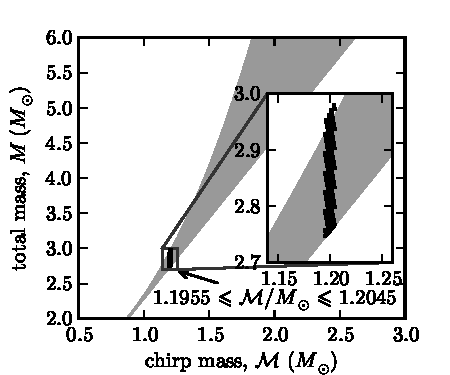
\includegraphics[width=1.1\textwidth]{figures/tmpltbank}
	\caption{\label{fig:tmpltbank}Source parameters for benchmark. Waveforms enter the Advanced {\small LIGO} band $\sim$\oldstylenums{17.5} minutes before merger.}
\end{figure}

\begin{figure}
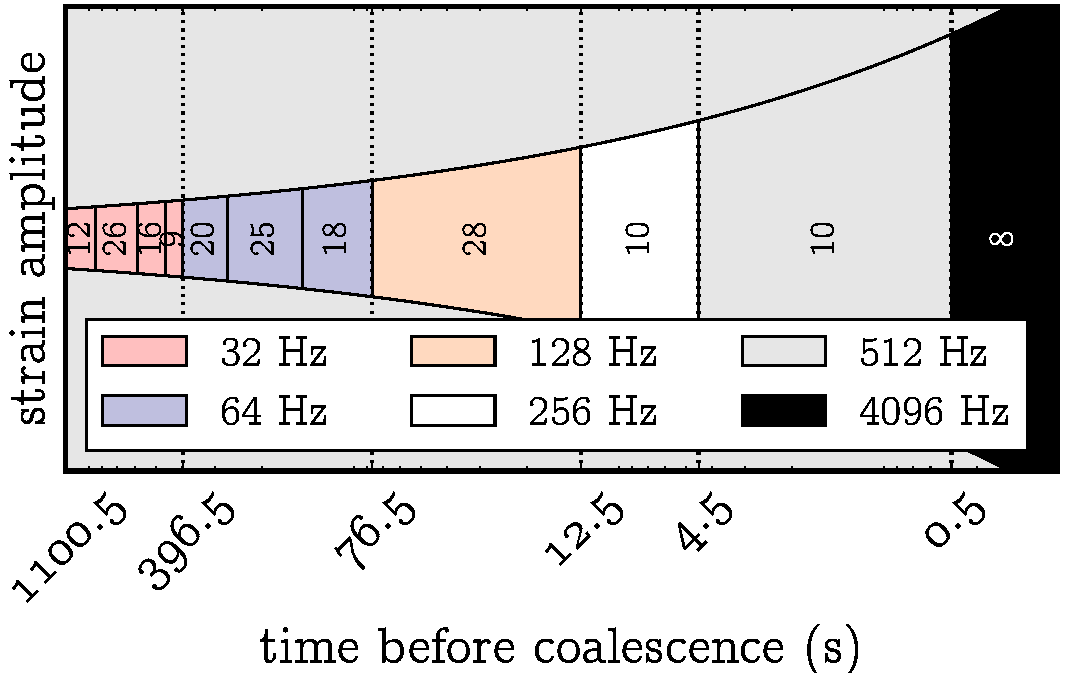
\includegraphics{figures/envelope}
\caption{\label{fig:time_slices} Representative waveform amplitude envelope with time slices color-coded by sample rate and annotated with the number of orthogonal templates.}
\end{figure}

%\vspace{-1.5em}
{\setlength{\parindent}{1em}
\gstreamer{} is an open-source framework used for
Linux desktop and mobile multimedia players. As ground-based interferometric
detectors are sensitive to \GW{}s at audio frequencies, \gstreamer{} happens to be
an excellent fit for low-latency \LIGO\ data analysis.
}
%
\begin{figure}
\includegraphics[width=\textwidth]{figures/network}
\caption{\label{fig:gstreamer}Visualization of part of a typical GStreamer pipeline.}
\end{figure}

\end{minipage}

\begin{minipage}[t]{0.33\textwidth}
%%% References
\bibliographystyle{apj}
\bibliography{references}
\end{minipage}%
\hspace{0.05\textwidth}%
\begin{minipage}[t]{0.62\textwidth}
\section*{Acknowledgements}

\LIGO\ was constructed by Caltech and \textsc{mit} with funding from the
\textsc{nsf} and operates under cooperative agreement
\textsc{phy}-\oldstylenums{0107417}. \textsc{ls} is supported by the
\textsc{nsf} through a Graduate Research Fellowship.
\newline\newline


\includegraphics[height=3cm]{figures/LSC_logo}\hspace{7.5mm}
\raisebox{-7.5mm}{
\includegraphics[height=4.5cm]{figures/Caltech_logo}}\hspace{7.5mm}
\raisebox{-7.5mm}{
\includegraphics[height=4.5cm]{figures/nsf1}}
\raisebox{1.5mm}{\includegraphics[height=3cm]{figures/gstreamer-logo}}
\newline\newline
\emph{Presented at {\small IAUS} \oldstylenums{285}, Oxford, UK, and LSC-Virgo Fall \oldstylenums{2011}, Gainesville, FL.} \\
This poster has \textsc{ligo} document number \LIGO{}-\textsc{g}\oldstylenums{1100683}-v\oldstylenums{4}.
\end{minipage}

\end{document}
